\newpage
\subsection{Diseño de interfaces de la aplicación móvil (UI/UX)}

La interfaz de la aplicación móvil EcoVerde fue desarrollada siguiendo los lineamientos de \textbf{Material Design 3}, el sistema de diseño de Google para aplicaciones Android.

\subsubsection{Diseño visual y prototipos de alta fidelidad}

 Este sistema proporciona componentes, colores y tipografía coherentes que garantizan una experiencia de usuario consistente y accesible.

\paragraph{Lenguaje de diseño.}
La paleta de colores se construyó a partir de un verde bosque (\texttt{\#2d6a3e}) como color principal, del cual se derivan los demás tonos de la interfaz. El color comunica el estado sanitario de forma directa: verde para árboles sanos, rojo para infestados y naranja para capturas sin resultado definitivo. La tipografía utilizada es \textbf{Roboto Flex}, tipografía oficial de Material Design 3. La aplicación soporta tema claro y oscuro para adaptarse a distintas condiciones de iluminación en campo.

Los prototipos presentados en las siguientes figuras representan el diseño final de cada pantalla de la aplicación.


\begin{figure}[H]
    \centering
    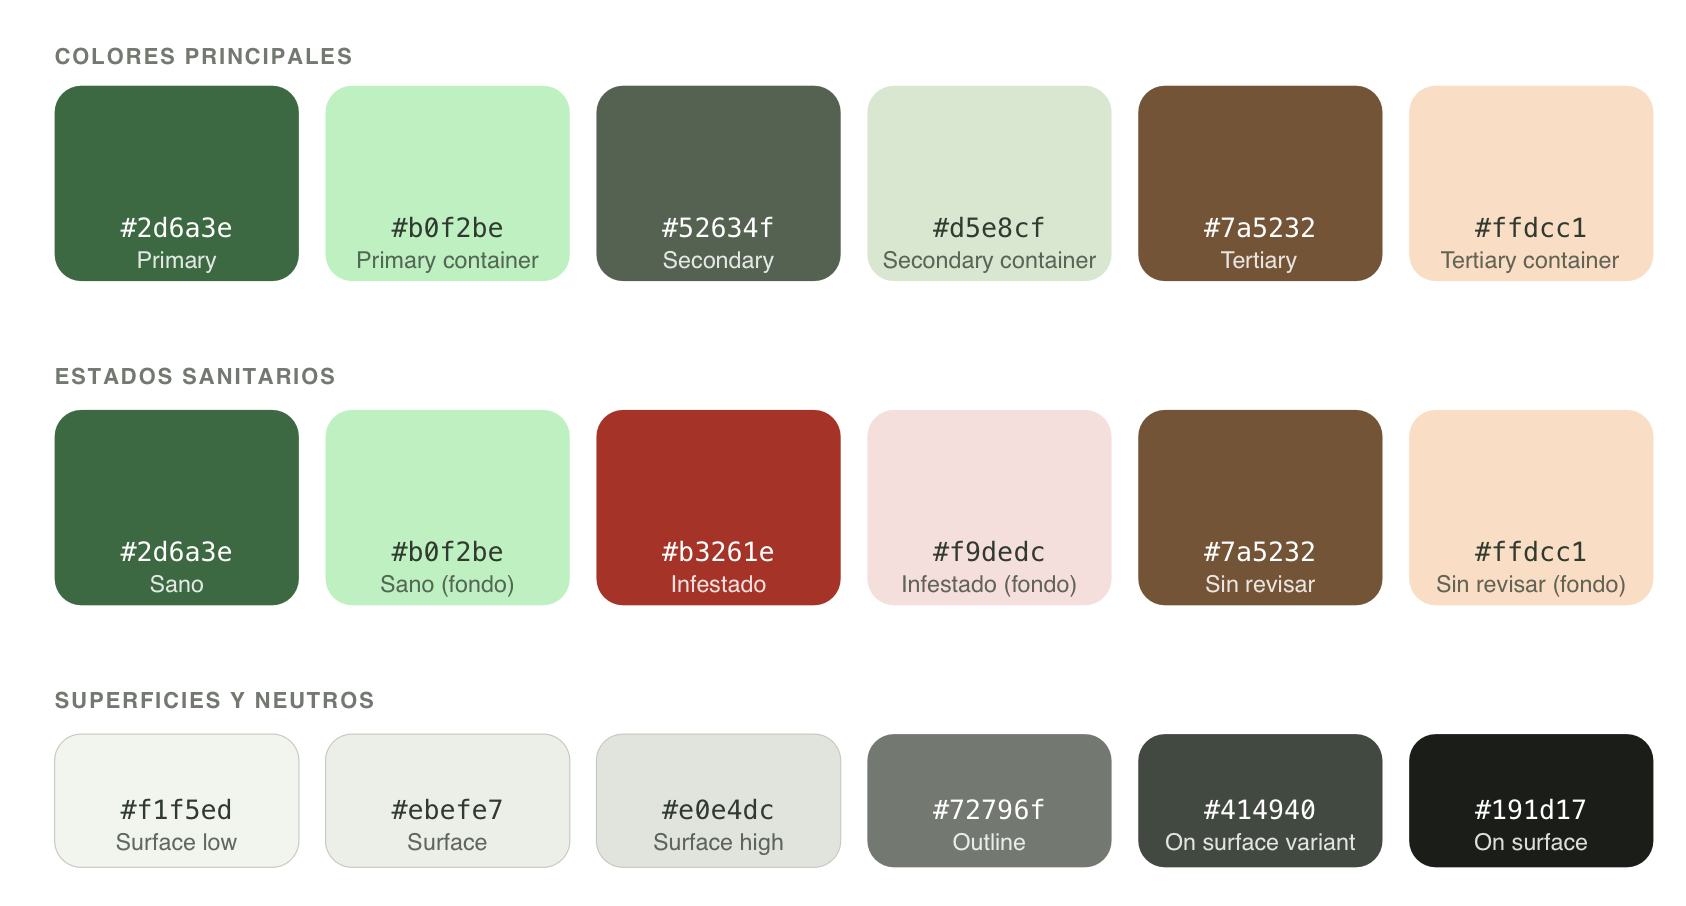
\includegraphics[width=1\textwidth]{images/Pantallas/color.png}
    \caption{Paleta de colores utilizada en el diseño.}
\end{figure}


% ── Figura 1 ──
\begin{figure}[H]
    \centering
    \begin{minipage}{0.35\textwidth}
        \centering
        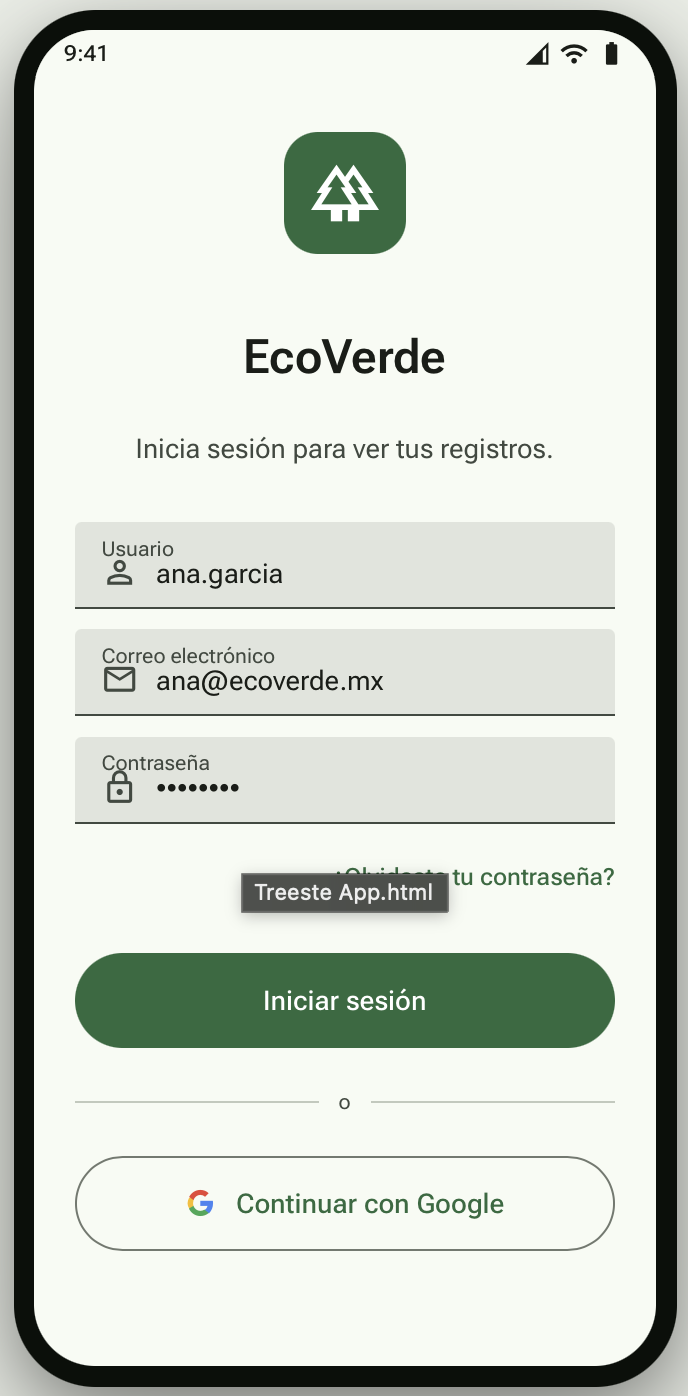
\includegraphics[width=\textwidth]{images/Pantallas/Movil/MOV1.png}
        \caption{Pantalla de inicio de sesión.}
        \label{fig:pantalla1}
    \end{minipage}
    \hfill
    \begin{minipage}{0.35\textwidth}
        \centering
        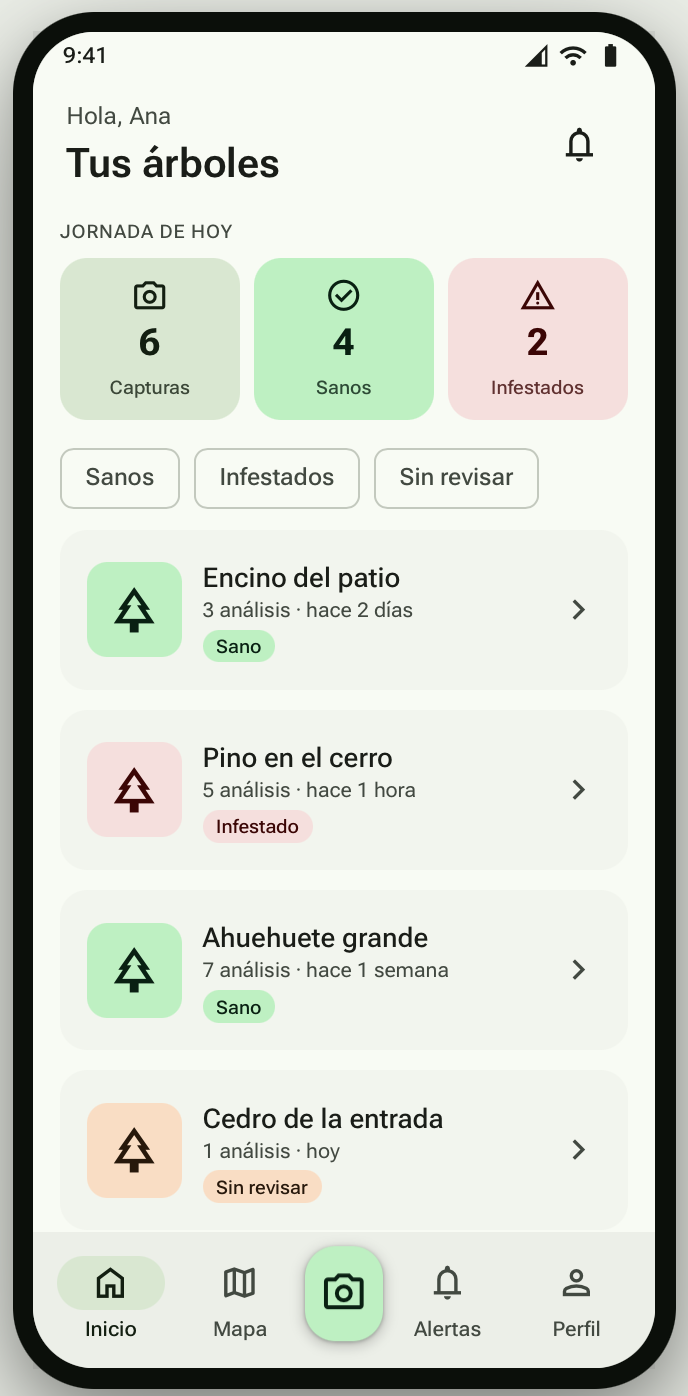
\includegraphics[width=\textwidth]{images/Pantallas/Movil/MOV3.png}
        \caption{Pantalla de creación de cuenta.}
        \label{fig:pantalla2}
    \end{minipage}
    \vspace{0.5cm}
    \begin{minipage}{0.35\textwidth}
        \centering
        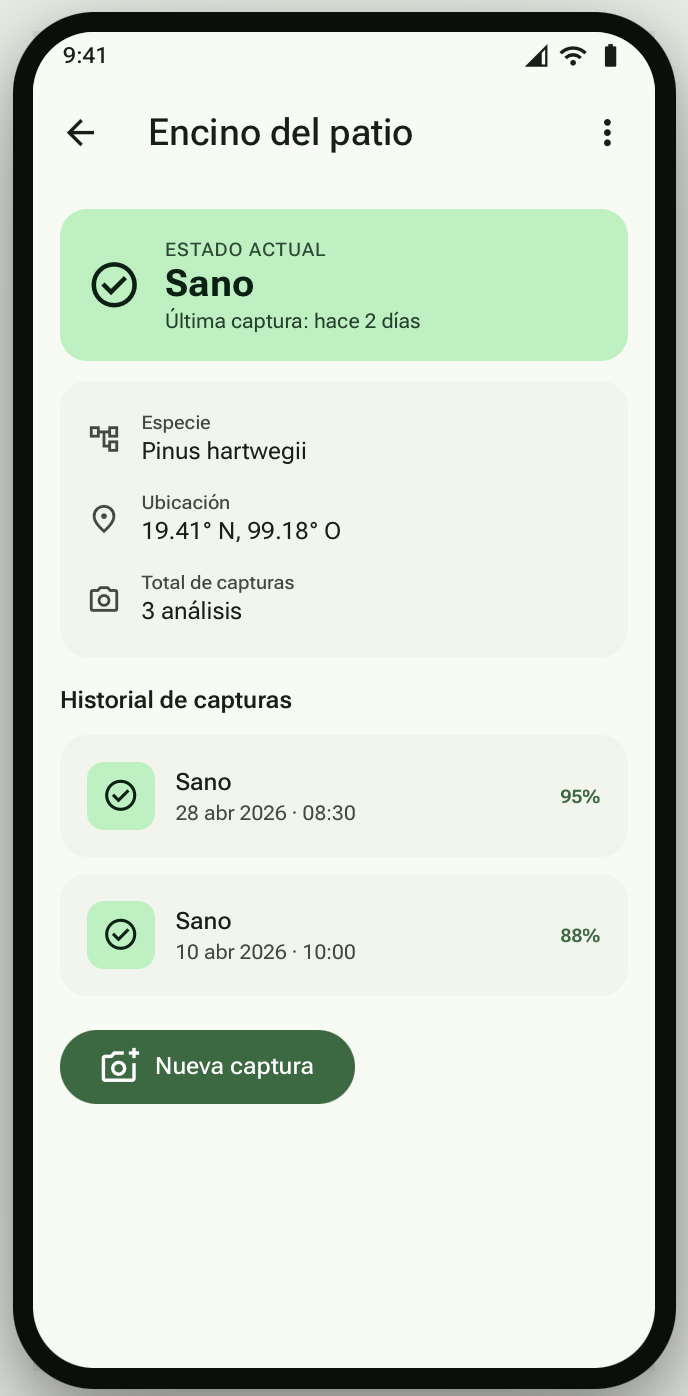
\includegraphics[width=\textwidth]{images/Pantallas/Movil/MOV4.png}
        \caption{Menú principal con resumen de jornada y lista de árboles registrados.}
        \label{fig:pantalla3}
        
    \end{minipage}
    \hfill
    \begin{minipage}{0.35\textwidth}
        \centering
        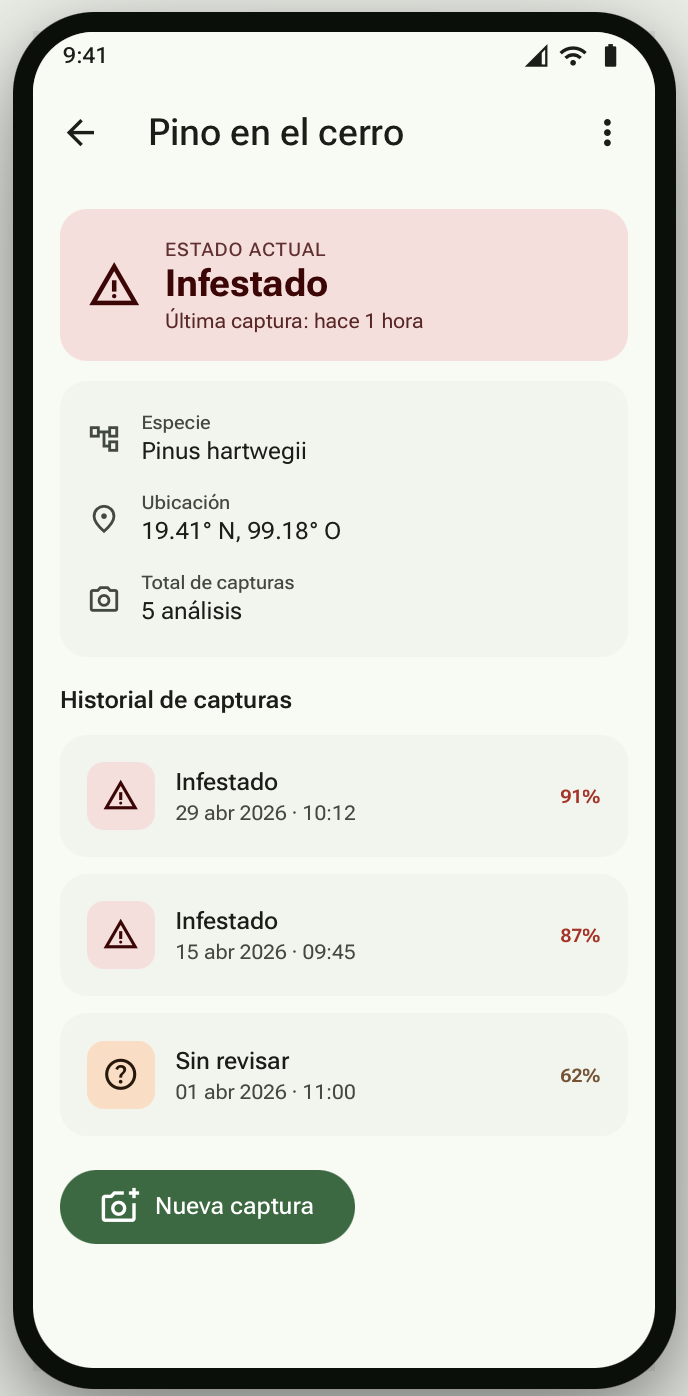
\includegraphics[width=\textwidth]{images/Pantallas/Movil/MOV5.png}
        \caption{Detalle de árbol: estado sanitario e historial de capturas.}
        \label{fig:pantalla4}
    \end{minipage}
\end{figure}

% ── Figura 2 ──
\begin{figure}[H]
    \centering
    \begin{minipage}{0.35\textwidth}
        \centering
        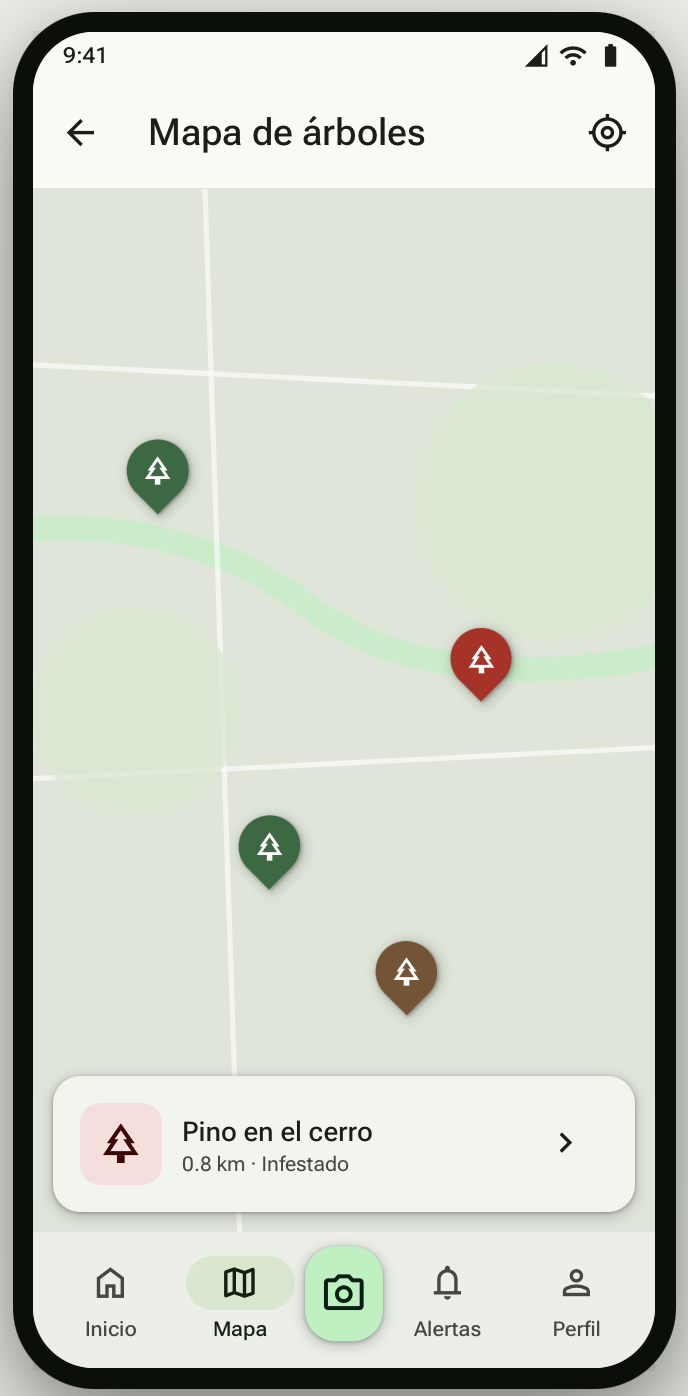
\includegraphics[width=\textwidth]{images/Pantallas/Movil/MOV6.png}
        \caption{Mapa de árboles registrados con indicadores de estado sanitario.}
        \label{fig:pantalla6}
    \end{minipage}
    \hfill
    \begin{minipage}{0.35\textwidth}
        \centering
        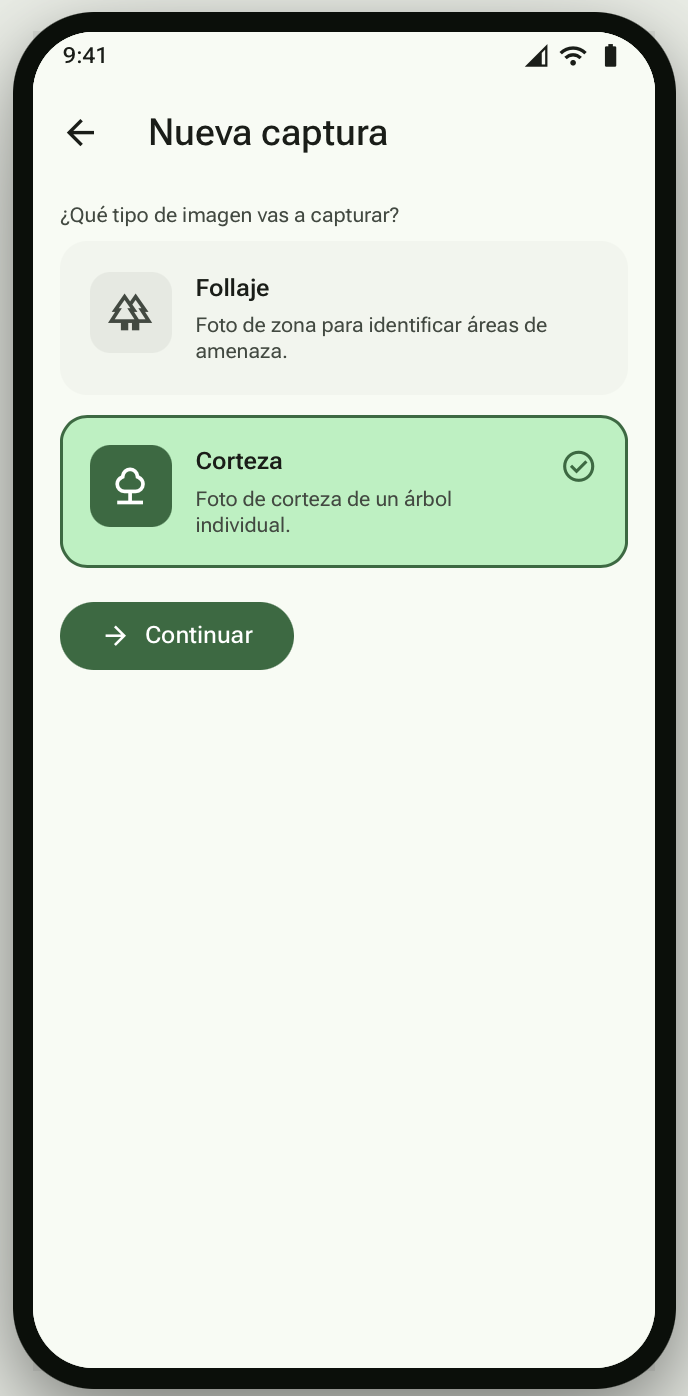
\includegraphics[width=\textwidth]{images/Pantallas/Movil/MOV7.png}
        \caption{Selección del tipo de captura: corteza o follaje.}
        \label{fig:pantalla7}
    \end{minipage}
    \vspace{0.5cm}
    \begin{minipage}{0.35\textwidth}
        \centering
        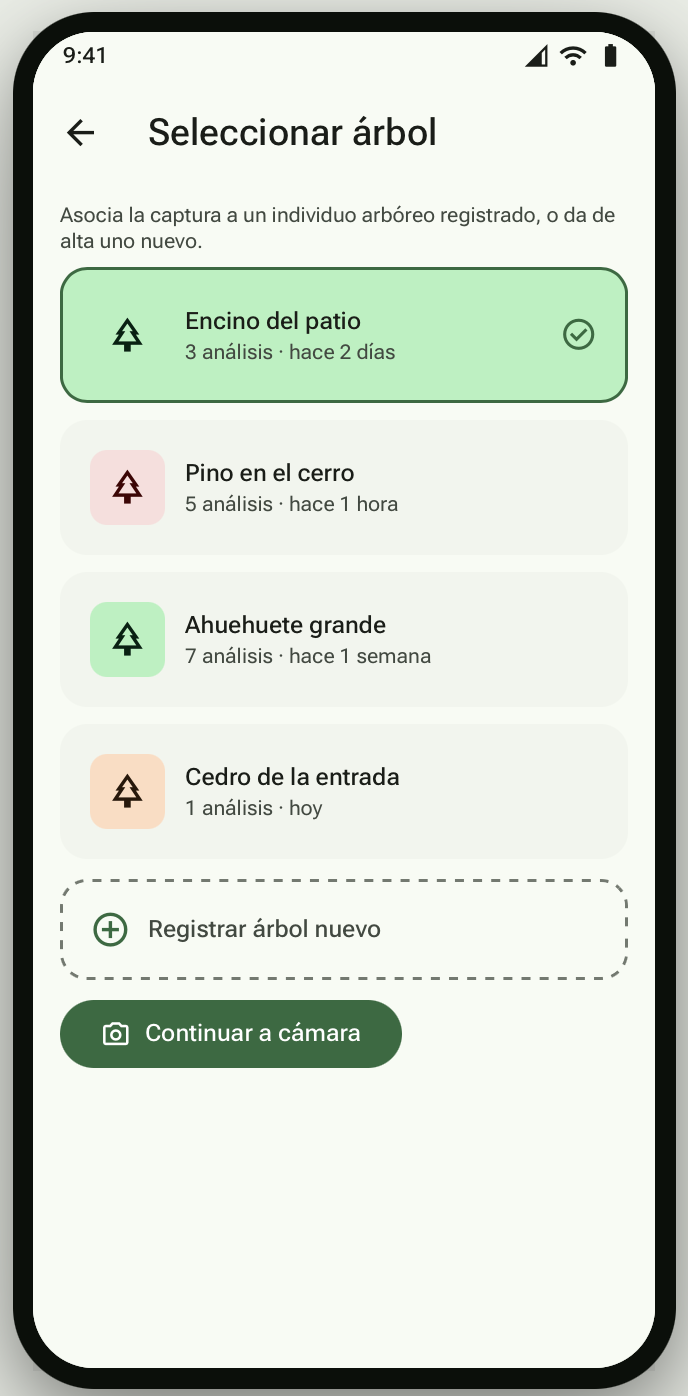
\includegraphics[width=\textwidth]{images/Pantallas/Movil/MOV8.png}
        \caption{Selección del árbol al que se asociará la captura.}
        \label{fig:pantalla8}
    \end{minipage}
    \hfill
    \begin{minipage}{0.35\textwidth}
        \centering
        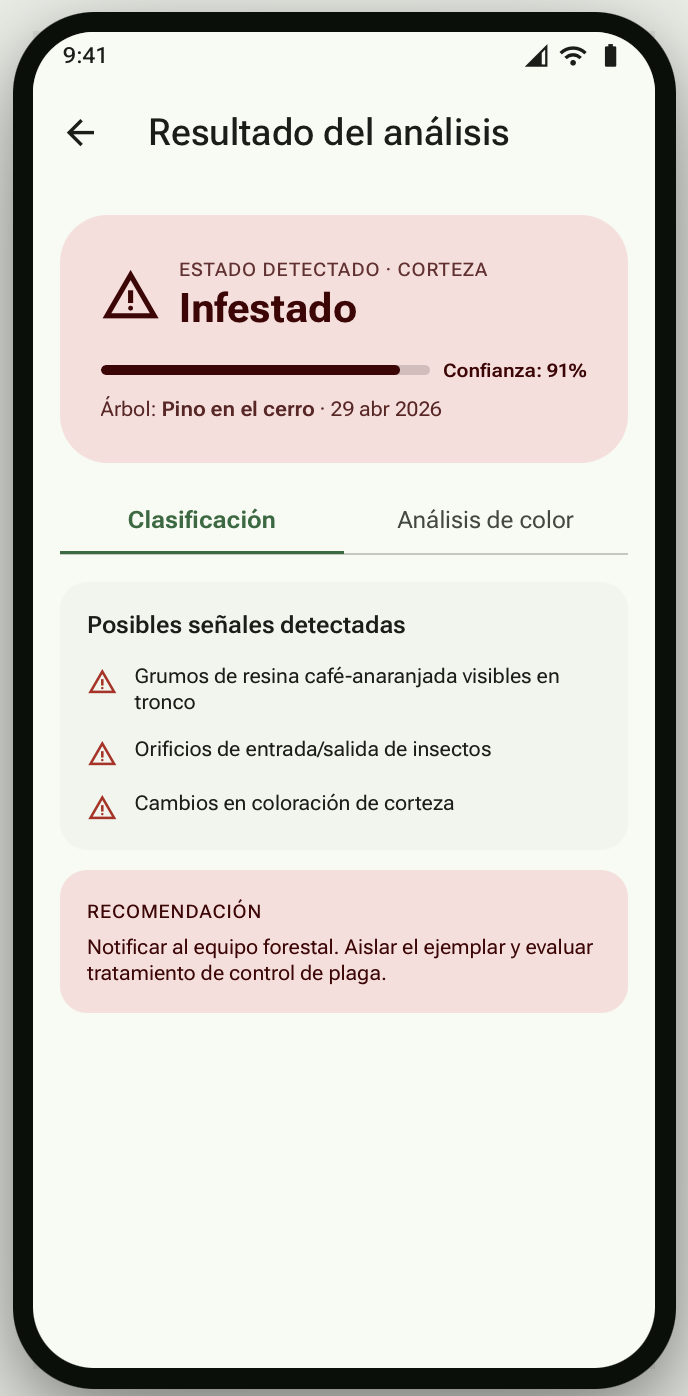
\includegraphics[width=\textwidth]{images/Pantallas/Movil/MOV9.png}
        \caption{Resultado del análisis de corteza: clasificación e índice de confianza.}
        \label{fig:pantalla9}
    \end{minipage}
\end{figure}

% ── Figura 3 ──
\begin{figure}[H]
    \centering
    \begin{minipage}{0.35\textwidth}
        \centering
        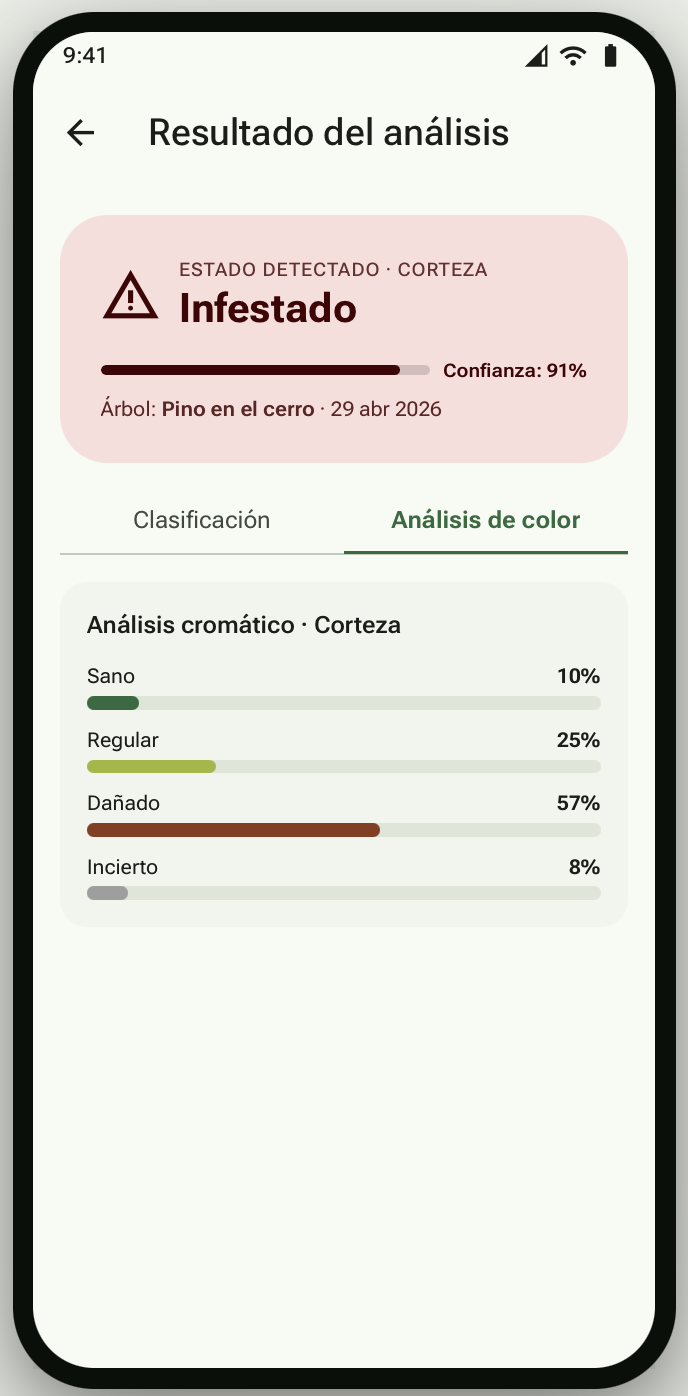
\includegraphics[width=\textwidth]{images/Pantallas/Movil/MOV10.png}
        \caption{Resultado del análisis de corteza: análisis de color.}
        \label{fig:pantalla10}
    \end{minipage}
    \hfill
    \begin{minipage}{0.35\textwidth}
        \centering
        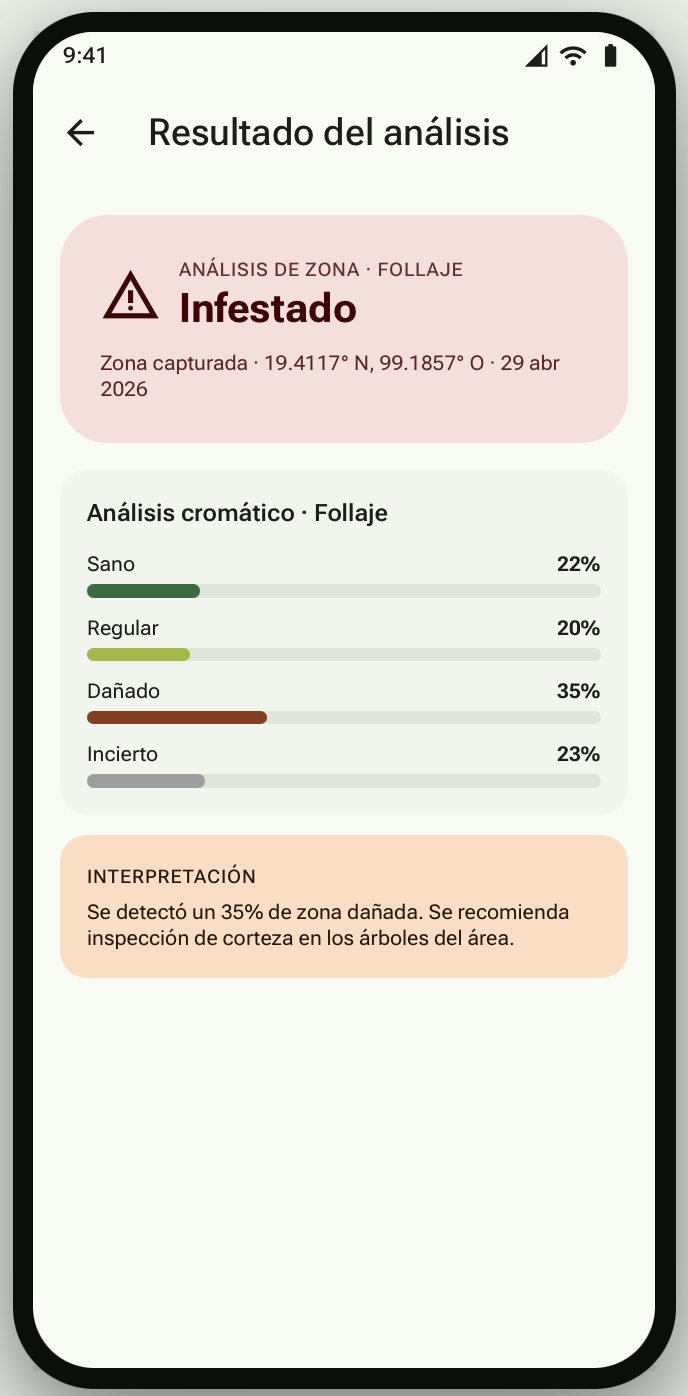
\includegraphics[width=\textwidth]{images/Pantallas/Movil/MOV11.png}
        \caption{Resultado del análisis de follaje: distribución cromática de la zona capturada.}
        \label{fig:pantalla11}
    \end{minipage}
    \vspace{0.5cm}
    \begin{minipage}{0.35\textwidth}
        \centering
        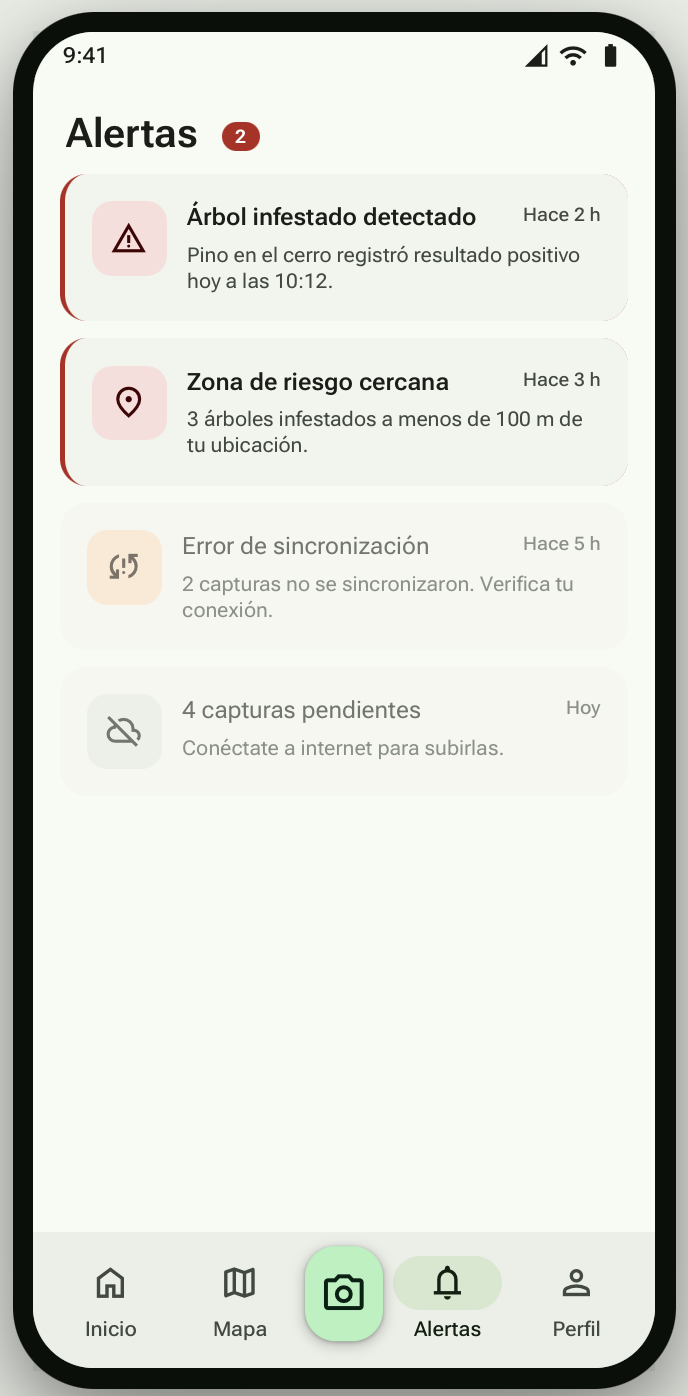
\includegraphics[width=\textwidth]{images/Pantallas/Movil/MOV12.png}
        \caption{Pantalla de alertas y notificaciones sanitarias.}
        \label{fig:pantalla12}
    \end{minipage}
    \hfill
    \begin{minipage}{0.35\textwidth}
        \centering
        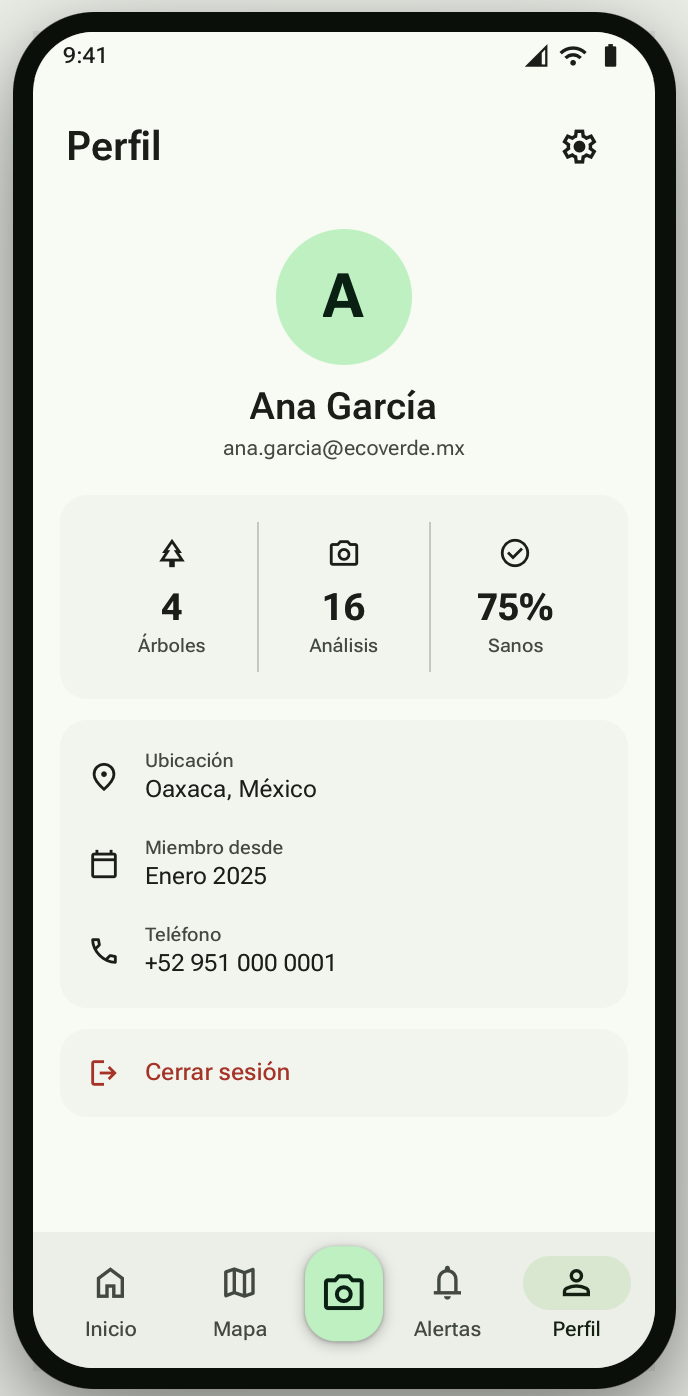
\includegraphics[width=\textwidth]{images/Pantallas/Movil/MOV13.png}
        \caption{Pantalla de perfil del técnico.}
        \label{fig:pantalla13}
    \end{minipage}
\end{figure}


% ─────────────────────────────────────────────────────────────
\subsubsection{Flujo de navegación y experiencia de usuario}

La navegación de EcoVerde está organizada en tres niveles:

\begin{enumerate}
    \item \textbf{Autenticación:} El técnico inicia sesión con correo y contraseña o mediante cuenta Google. Un flujo de incorporación de tres pasos presenta las funciones principales de la aplicación antes del primer acceso.

    \item \textbf{Navegación principal:} Una barra de navegación inferior permite acceder a las secciones de \textit{Inicio}, \textit{Mapa}, \textit{Alertas} y \textit{Perfil}. El botón central activa el flujo de nueva captura, siendo la acción más frecuente durante la jornada de campo.

    \item \textbf{Flujo de captura:} Consta de cuatro pasos secuenciales:
    \begin{enumerate}
        \item Selección del tipo de muestra: corteza o follaje.
        \item Asociación a un árbol registrado, o registro de uno nuevo (solo para corteza).
        \item Captura fotográfica con guía de encuadre en pantalla.
        \item Presentación del resultado del análisis.
    \end{enumerate}
\end{enumerate}


% ─────────────────────────────────────────────────────────────
\subsubsection{Presentación de resultados}

La pantalla de resultados traduce la salida del modelo de inferencia en información directamente útil para el técnico. Su contenido varía según el tipo de captura.

\paragraph{Resultado de corteza.}
Se muestra la clasificación del árbol (\textit{Sano}, \textit{Infestado} o \textit{Sin revisar}), el índice de confianza del modelo, las señales visuales detectadas en la imagen y una recomendación de acción. Una pestaña adicional presenta el análisis cromático de la corteza.

\paragraph{Resultado de follaje.}
Al tratarse de una captura de zona y no de un árbol individual, se presenta únicamente el análisis cromático de la imagen, con la distribución porcentual de superficie sana, regular, dañada e incierta. La ubicación geográfica de la captura queda registrada en el encabezado para su posterior consulta en el mapa.